\section{Cơ sở lý thuyết về Thị giác Máy tính (Computer Vision - CV)}

Phần này cung cấp kiến thức nền tảng và tổng quan về lĩnh vực Thị giác Máy tính, bao gồm định nghĩa, quy trình làm việc cơ bản (pipeline), các mô hình học sâu cốt lõi và phương pháp đánh giá hiệu suất. Những kiến thức này là cơ sở lý thuyết quan trọng, sẽ được tham chiếu trực tiếp trong phần ứng dụng về Ước lượng Tư thế Người và nền tảng MediaPipe ở phần tiếp theo.

\subsection{Định nghĩa và Mục tiêu}
\textbf{Thị giác Máy tính (Computer Vision, CV)} là một lĩnh vực liên ngành của Trí tuệ Nhân tạo (AI) cho phép máy tính thu nhận, xử lý, phân tích, và diễn giải hình ảnh hoặc video để đạt được khả năng ``hiểu'' nội dung ở cấp độ cao, tương tự thị giác con người. Mục tiêu chính là mô phỏng và vượt qua khả năng nhận thức thị giác của con người về tốc độ, độ chính xác, và quy mô.\autocite{szeliski2010} Hình ảnh kỹ thuật số là ma trận số: ảnh xám là ma trận 2D với giá trị cường độ từ 0 đến 255, còn ảnh màu là ma trận 3D (chiều cao $\times$ chiều rộng $\times$ 3 kênh RGB). Thông tin ý nghĩa (như vật thể, cạnh, hoặc vùng) nằm trong cách sắp xếp và biến đổi gradient của các giá trị pixel này.\autocite{lowe1999} Ví dụ, từ dữ liệu pixel, hệ thống có thể tái tạo mô hình 3D hoặc phân tích chuyển động.

\subsection{Pipeline Cơ bản của Hệ thống CV}
Một hệ thống Thị giác Máy tính điển hình hoạt động theo quy trình tuần tự như Hình~\ref{fig:cv_pipeline}:

\begin{figure}[h]
    \centering
    \includegraphics[width=0.9\textwidth]{vision_flow-crop.pdf}
    \caption{Quy trình tổng thể của một hệ thống Thị giác Máy tính từ ảnh đầu vào đến kết quả phân tích.}
    \label{fig:cv_pipeline}
\end{figure}

\begin{enumerate}
    \item \textbf{Thu nhận dữ liệu}  
    Thu thập hình ảnh tĩnh hoặc chuỗi video từ camera/cảm biến (RGB, hồng ngoại hoặc 3D), đảm bảo chất lượng và độ phân giải phù hợp.\autocite{szeliski2010}
    
    \item \textbf{Tiền xử lý}  
    Chuẩn bị dữ liệu số cho phân tích bằng các bước:
    \begin{itemize}
        \item \emph{Giảm nhiễu}: Lọc Gaussian: 
        \[
            I_{\text{filtered}} = \text{Gaussian}(I, \sigma)
        \]
        \item \emph{Chuẩn hóa pixel}: giá trị pixel về [0,1] hoặc cân bằng histogram để điều chỉnh độ sáng.
        \item \emph{Chuyển đổi không gian màu}: RGB $\to$ HSV hoặc thang xám để tách màu, độ bão hòa, và giá trị sáng.
    \end{itemize}\autocite{szeliski2010}
    
    \item \textbf{Trích xuất đặc trưng}  
    Biến dữ liệu pixel thành đặc trưng có ý nghĩa:
    \begin{itemize}
        \item \textbf{Cạnh}: Phát hiện thay đổi cường độ đột ngột bằng gradient:
        \[
            G = \sqrt{G_x^2 + G_y^2}, \quad
            G_x = \frac{\partial I}{\partial x}, \quad
            G_y = \frac{\partial I}{\partial y}
        \]
        Hoặc dùng thuật toán Canny (lọc Gaussian, non-max suppression, hysteresis).\autocite{sobel1968,canny1986}
        
        \item \textbf{Điểm đặc trưng}:  
        \begin{itemize}
            \item Harris: tìm góc dựa trên ma trận tự tương quan, eigenvalue $\lambda_1, \lambda_2$ lớn.
            \item SIFT: đặc trưng bất biến theo quy mô qua Difference of Gaussians (DoG).\autocite{lowe1999}
        \end{itemize}

        \item \textbf{Mô tả toàn cục}:
        \begin{itemize}
            \item HOG: Histogram hướng gradient phân tích hướng cạnh.
            \item LBP: Local Binary Patterns mã hóa nhị phân lân cận pixel.\autocite{dalal2005}
        \end{itemize}
    \end{itemize}
    
    \item \textbf{Phân tích và ra quyết định}  
    Dựa trên đặc trưng, mô hình thực hiện phân loại, nhận dạng hoặc ước lượng tư thế. Kết quả có thể là nhãn, hộp giới hạn, hoặc hành động (ví dụ: xe tự hành dừng khi phát hiện chướng ngại).\autocite{horn1981}
\end{enumerate}

\subsection{Phân loại các Bài toán CV Cốt lõi}
Các bài toán trong CV được phân loại dựa trên mức độ chi tiết của đầu ra:

\begin{itemize}
    \item \textbf{Phân loại Ảnh}: Gán nhãn duy nhất cho toàn bộ hình ảnh (ví dụ: ``Xe hơi'', ``Người'').\autocite{krizhevsky2012}
    \item \textbf{Phát hiện Đối tượng}: Xác định vị trí nhiều đối tượng bằng hộp giới hạn và gán nhãn.\autocite{redmon2016}
    \item \textbf{Phân đoạn Ảnh}:
    \begin{itemize}
        \item \textbf{Phân đoạn Ngữ nghĩa}: Phân loại từng pixel (ví dụ: Đường, Bầu trời).\autocite{ronneberger2015}
        \item \textbf{Phân đoạn Thể hiện}: Phân biệt các cá thể cùng lớp (ví dụ: Người 1, Người 2).\autocite{ronneberger2015}
    \end{itemize}
    \item \textbf{Ước lượng Tư thế Người}: Xác định tọa độ các khớp keypoint trên cơ thể, nền tảng cho phân tích chuyển động.\autocite{lin2014}
\end{itemize}

\subsection{Các Mô hình Học sâu Cốt lõi trong CV Hiện đại}
\subsubsection{Mạng Nơ-ron Tích chập (Convolutional Neural Networks - CNN)}
CNN là kiến trúc chủ đạo, tự động học đặc trưng phân cấp qua các lớp tích chập và gộp:

\begin{itemize}
    \item \textbf{Phép Tích chập}: Trích xuất đặc trưng cục bộ: $(I * K)(i, j) = \sum_{m} \sum_{n} I(i-m, j-n) K(m, n)$, với $K$ là kernel, $I$ là ảnh đầu vào.\autocite{lecun1998}
    \item \textbf{Phép Gộp}: Giảm kích thước không gian, ví dụ Max Pooling:
\[
O_{i,j} = \max \bigl( I_{2i,\,2j},\; I_{2i+1,\,2j},\; I_{2i,\,2j+1},\; I_{2i+1,\,2j+1} \bigr)
\]
\autocite{lecun1998}
    \item \textbf{Kiến trúc nổi bật}: AlexNet, VGG, ResNet (dùng Residual Block), YOLO (phát hiện thời gian thực).\autocite{krizhevsky2012,simonyan2014,he2016,redmon2016} Autoencoder nén dữ liệu để học biểu diễn ẩn.\autocite{szeliski2010}
\end{itemize}

\begin{figure}[h]
    \centering
    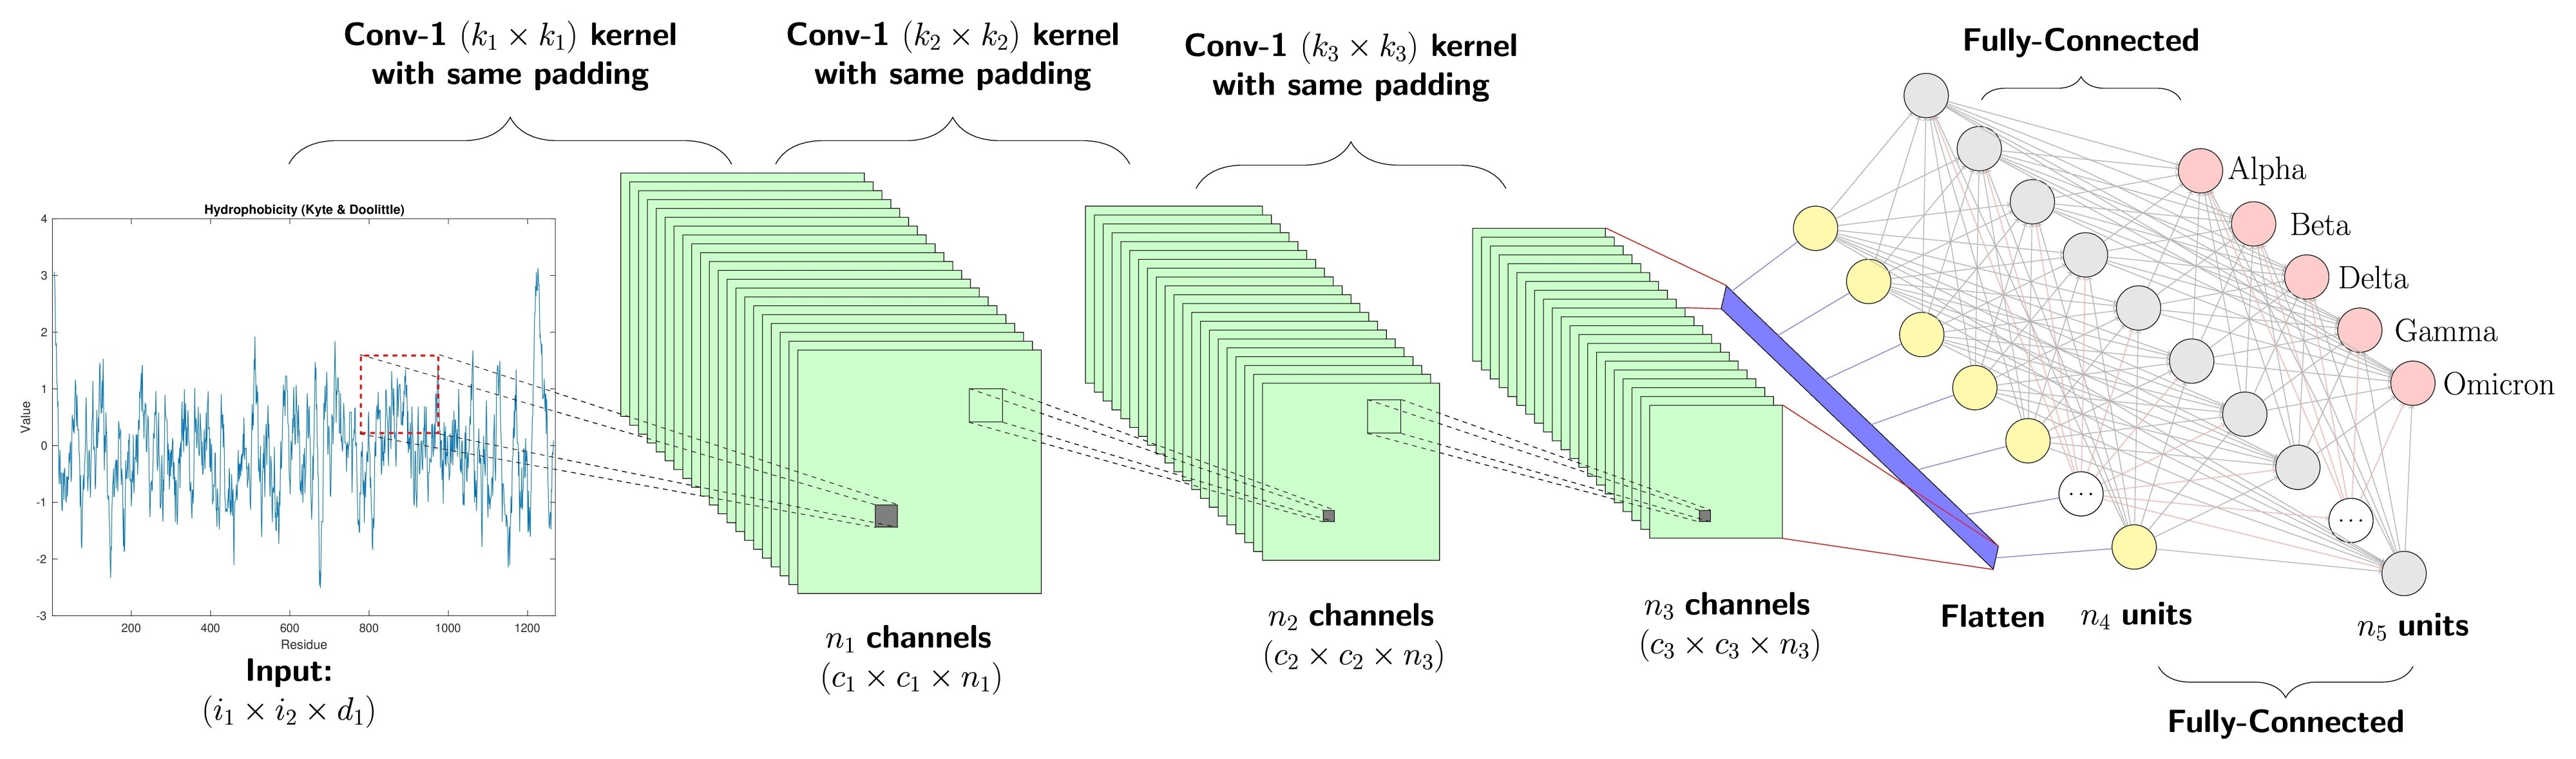
\includegraphics[width=0.8\textwidth]{2_2_convolution.jpeg}
    \caption{Minh họa các phép toán tích chập và gộp trong CNN.}
    \label{fig:cnn_ops}
\end{figure}

\subsubsection{Mô hình dựa trên Transformer}
Vision Transformer (ViT) chia ảnh thành các miếng vá, xử lý như chuỗi token, sử dụng cơ chế Self-Attention: $\text{Attention}(Q, K, V) = \text{softmax}\left(\frac{QK^T}{\sqrt{d_k}}\right)V$, với $Q, K, V$ là ma trận Query, Key, Value.\autocite{dosovitskiy2021} ViT vượt qua giới hạn cục bộ của CNN bằng cách học mối quan hệ toàn cục.

\begin{figure}[h]
    \centering
    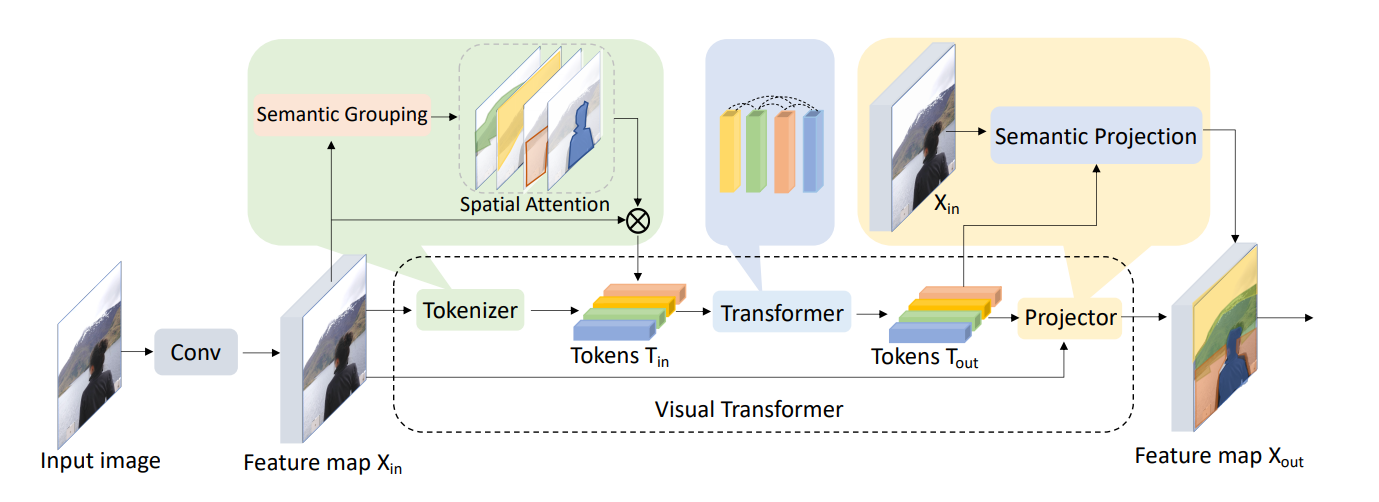
\includegraphics[width=0.9\textwidth]{visual_transformer.png}
    \caption{Kiến trúc Vision Transformer chuyển đổi hình ảnh thành chuỗi token.}
    \label{fig:vit_arch}
\end{figure}

\subsubsection{Mô hình Phân tích Cấp cao}
U-Net dùng encoder-decoder cho phân đoạn pixel-wise.\autocite{ronneberger2015} Optical flow (Horn-Schunck) tính chuyển động: $I_x u + I_y v + I_t = 0$.\autocite{horn1981} Quyết định dựa trên SVM hoặc ngưỡng trên đặc trưng.\autocite{szeliski2010}

\subsection{Các tập dữ liệu phổ biến và thước đo đánh giá mô hình}
\begin{itemize}
    \item \textbf{Tập dữ liệu}:
    \begin{itemize}
        \item ImageNet: Hơn 14 triệu ảnh, 20,000 lớp.\autocite{deng2009}
        \item COCO: Phát hiện và phân đoạn đối tượng.\autocite{lin2014}
        \item MPII, COCO Keypoints: Ước lượng tư thế người.\autocite{lin2014}
    \end{itemize}
    \item \textbf{Metrics}:
    \begin{itemize}
        \item IoU: $\frac{\text{Area of Overlap}}{\text{Area of Union}}$.\autocite{lin2014}
        \item mAP: Trung bình Average Precision trên các lớp.\autocite{lin2014}
        \item F1-score: Trung bình điều hòa Precision và Recall.\autocite{szeliski2010}
        \item OKS: Đo lường độ chính xác khớp trong HPE.\autocite{lin2014}
    \end{itemize}
\end{itemize}

Ví dụ thực tế: Hệ thống tự lái dùng CNN để nhận diện làn đường từ cạnh và gradient, kết hợp optical flow để dự đoán chuyển động.\autocite{redmon2016}
